\section{Operations} \label{sec:ECAL_Operations}

In order to take take quality data at the CMS ECAL and test the re-optimized and new features of the ECAL trigger for LHC Run 3, a variety of operations teams is necessary. The CMS ECAL operations are subdivided into various operations groups, as there is a wide array of areas of technology and expertise required in order to successfully operate the ECAL for data-taking. Each group covers a different aspect of ECAL, all with the goal of minimizing the downtime of the experiment and ensuring quality data is taken. There are many sides to the operation of ECAL, for each of which the corresponding operations team is crucial, and all must remain vigilant for the successful operation and maintenance of ECAL. 

\subsection{Technical Coordination}

The purpose of the ECAL Technical Coordination (TC) is to ensure the safe operation of all hardware components of ECAL, both those stored in the Underground Experimental Cavern (UXC), and Underground Service Cavern (USC). In the event of a major hardware failure, or cooling related issue which may occur and possibly prevent ECAL from running in a safe state, the TC team leads the effort in repairing these components and is responsible for notifying the rest of the ECAL operations group that a particular partition of ECAL is unavailable. During periods of collisions, and especially during long shutdown or technical stop periods, CMS TC coordinates a vast number of physical interventions to repair, upgrade, and service the detector. This large coordination effort requires a deep understanding of the physical architecture and history of ECAL, as well as an understanding of how an intervention on one CMS subdetector may affect another CMS subdetector. The role of the ECAL TC team includes following the planned CMS TC activities, as this may have implications on partitions of ECAL. An example CMS underground plan of the day is shown in Figure \ref{fig:CMS_TC_Example}.

\begin{figure}[H]
    \centering
    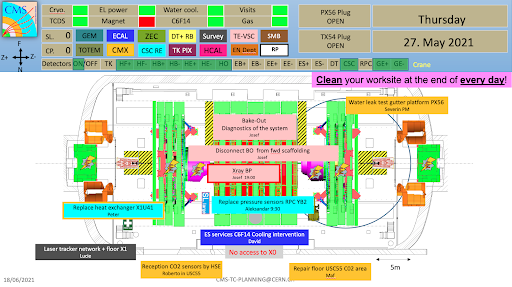
\includegraphics[width=0.85\textwidth]{Images/ECAL_Operations/CMS_TC_Example.png}
    \caption{Example plan of the day in CMS UXC/USC from 27 May 2021.}
    \label{fig:CMS_TC_Example}
\end{figure}

As an example, during a long LHC shutdown period there may be a day when one of the CMS endcaps must be physically moved in order to allow for an intervention on the inner hardware of another sub-detector which is not accessible when the detector is closed. This has an implication of the ECAL endcaps, as they may need to be powered off during this time to ensure the safety of the electronics. In a case like this, ECAL TC would report this required action of powering off to the rest of the ECAL operations teams in order for all to be aware that one endcap will not be available for a certain period of time. This can then potentially delay planned tests on this endcap, and is therefore essential information for the entire ECAL operations group to be aware of. 

\subsection{Detector Control System}

% https://indico.cern.ch/event/1122238/contributions/4711434/attachments/2380818/4067982/TrainingSession%20ECAL%20DCS%20Operators.pdf

The ECAL Detector Control System (DCS) team maintains, develops, and operates the ECAL DCS in order to ensure the proper control and safety of the detector. An image of the ECAL DCS monitor is shown in Figure \ref{fig:ECAL_DCS_Monitor}, displaying the powering status of the full ECAL and ES as ON. 

\begin{figure}[H]
    \centering
    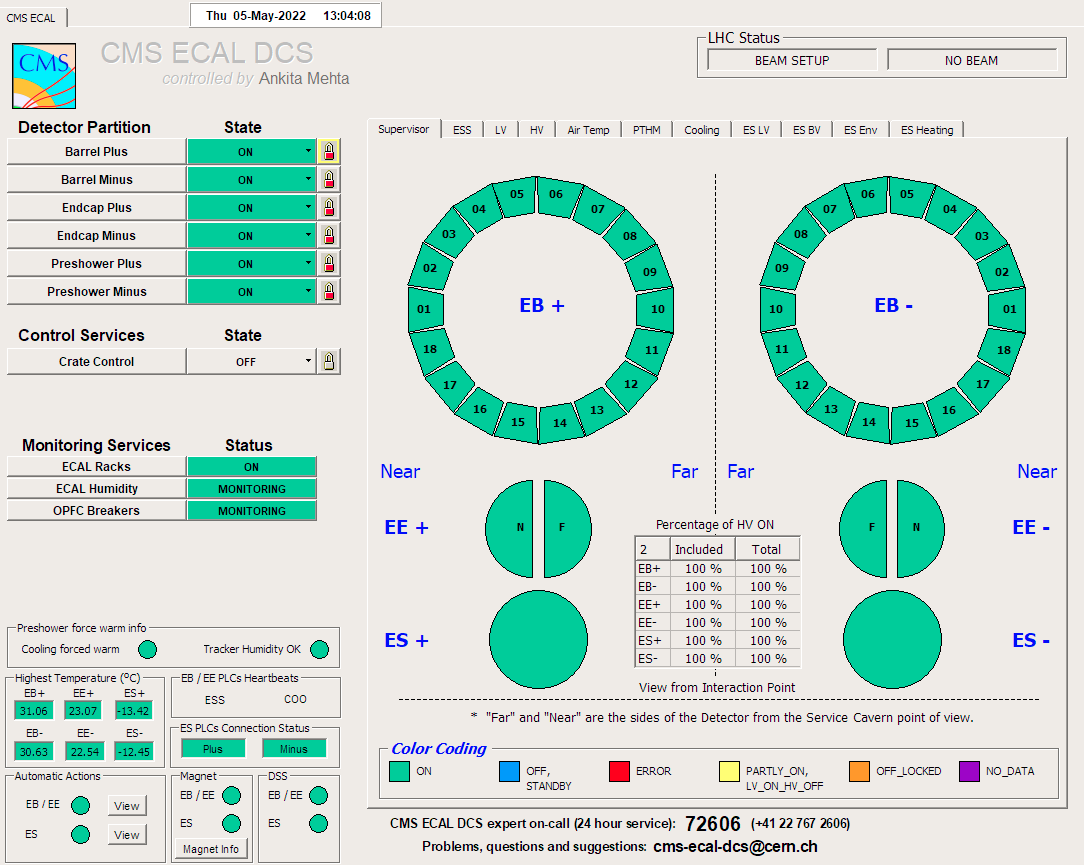
\includegraphics[width=0.85\textwidth]{Images/ECAL_Operations/ECAL_DCS.png}
    \caption{ECAL DCS monitor}
    \label{fig:ECAL_DCS_Monitor}
\end{figure}

In the example situation in which there is activity in UXC which requires the powering off of an ECAL Endcap, a request would be made to the ECAL DCS operator to use the DCS in order to power off the desired partition of ECAL. In the event in which issues during this powering off may occur, the operator follows a pre-defined set of protocols in order to safely identify and solve the encountered issue without harming the detector.  

\subsection{Run Coordination}

The purpose of ECAL Run Coordination (RC) is to coordinate the running operations of ECAL, including all times during which the detector is powered on. This primarily involves the planning of tests, coordination between ECAL and CMS, and training of on-call ECAL shifters in order to carry out operation plans. A diagram illustrating the paths of communication between ECAL and CMS during running can be seen in Figure \ref{fig:ECAL_CMS_RC_diagram}.

\begin{figure}[H]
    \centering
    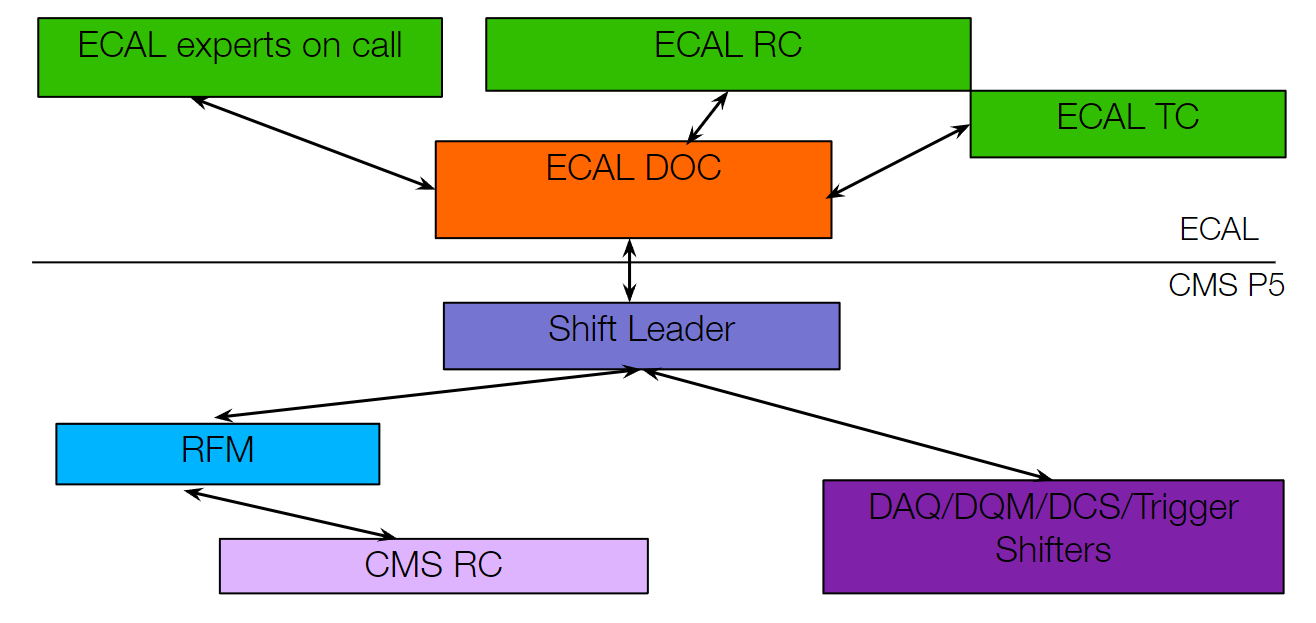
\includegraphics[width=0.85\textwidth]{Images/ECAL_Operations/ECAL_RC_Diagram.png}
    \caption{ECAL / CMS running communication paths.}
    \label{fig:ECAL_CMS_RC_diagram}
\end{figure}

On a given day, the CMS run coordinators and Run Field Manager (RFM) make a plan of the day based on the plan of LHC and the requests of the individual subdetectors. It is the job of ECAL RC to make sure the requests made to CMS are consistent with the opinions and availability of the ECAL experts, and to then understand and share the implications of the CMS plan of the day on the ECAL subdetector. This may include planned tests for ECAL which use the CMS DAQ (Data AcQuisition) system, or the participation of ECAL in the tests of other CMS subsystems. It is essential for all participants in run coordination communications to execute fast and clear communication of information in order to minimize detector downtime, and optimize the use of commissioning and data-taking periods. 

\subsection{Data Acquisition} \label{sec:ECAL_DAQ}

% https://indico.cern.ch/event/1122210/contributions/4711234/attachments/2394725/4094305/ECAL_DAQ_Tutorial_for_DOCs_2021.pdf
% https://ecal-daq-doc.docs.cern.ch/
% https://gitlab.cern.ch/ecal-daq/ecal-daq-documentation/-/tree/master/docs/images

The ECAL DAQ (Data AcQuisition) team is responsible for ensuring effective data-taking by ECAL. A diagram of the ECAL DAQ path is shown in Figure \ref{fig:ECAL_DCC_Diagram}. 

\begin{figure}[H]
    \centering
    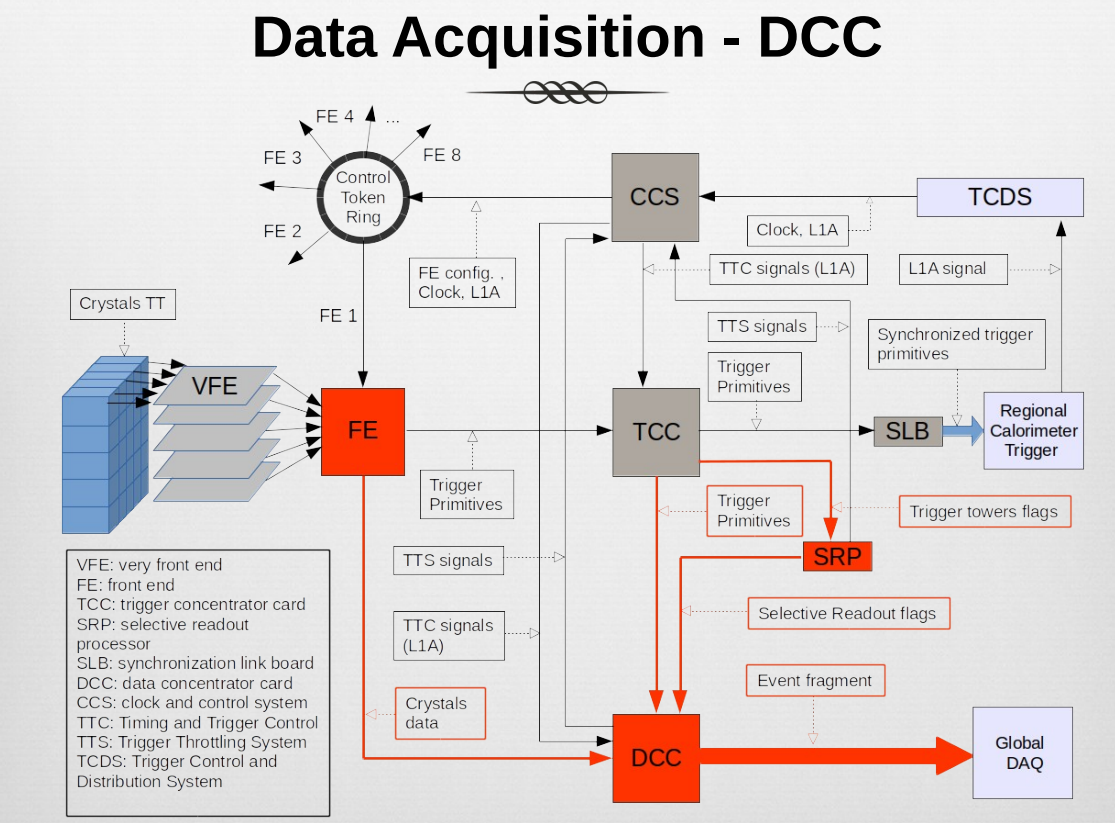
\includegraphics[width=0.85\textwidth]{Images/ECAL_Operations/ECAL_DCC_Diagram.png}
    \caption{ECAL DAQ path}
    \label{fig:ECAL_DCC_Diagram}
\end{figure}

Generally speaking, the data flow which takes place due to an energetic ECAL goes as follows: An energetic electromagnetically interacting particle produces scintillation light in the ECAL crystals (left-most side of Figure \ref{fig:ECAL_DCC_Diagram}), which reaches the crystals' photo-detectors (or an EB APD may be directly struck, leading to a spike which may fake an energetic ECAL signal). The signals from the photo-detectors are propagated through the VFE (very front end) cards, where in EB a set of five cards is connected to a single FE (front end card) for a 25 crystal TT, or a range of 1-25 crystals in EE. If an L1A is sent to the FE based on the CMS L1 trigger, the L1A will be received via the control token ring, triggering ECAL to readout its data first sending it to the DCC (data concentrator card), and then to the central CMS DAQ system to be processed at HLT. 

The ECAL DAQ team is additionally responsible for maintaining a slew of monitors used for monitoring various DAQ related quantities, to ensure that data acquisition is flowing as expected. An example is the ECAL payload monitor, used to monitor if very large amounts of data are being processed through each ECAL FED (Front end driver), corresponding to different parts of the detector (one supermodule in EB). The contents of this monitor during an ECAL full readout run, during a special run in which ECAL was running with double weights in tagging mode with the $\delta_{min}$ = 2.5 GeV working point as described in Section \ref{sec:ECALTrigger_Run3}, is shown in Figure \ref{fig:PayloadMonitor_ECAL} for ECAL, and \ref{fig:PayloadMonitor_ES} for the preshower.

\begin{figure}[H]
    \centering
    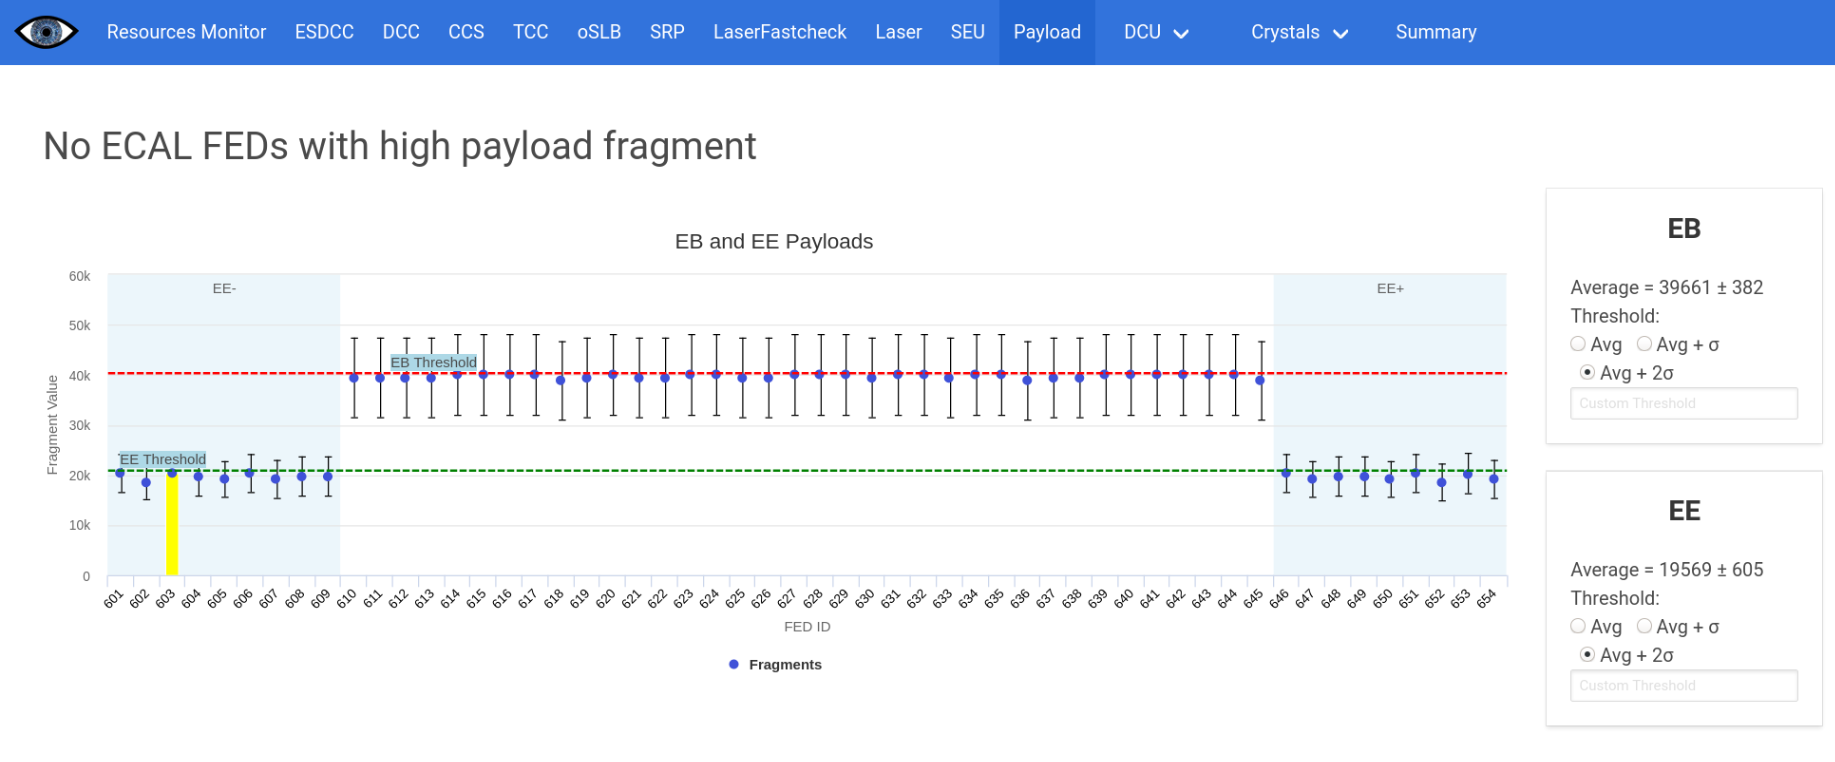
\includegraphics[width=\textwidth]{Images/ECAL_Operations/PayloadMonitor.png}
    \caption{ECAL payload monitor during a June 2022 full-readout run. On the y-axis, the size of a FED's payload fragment is plotted. On the x-axis, the ECAL FED number is plotted. Each FED number corresponds to an ECAL supermodule, and ranges from 601-654.}
    \label{fig:PayloadMonitor_ECAL}
\end{figure}

\begin{figure}[H]
    \centering
    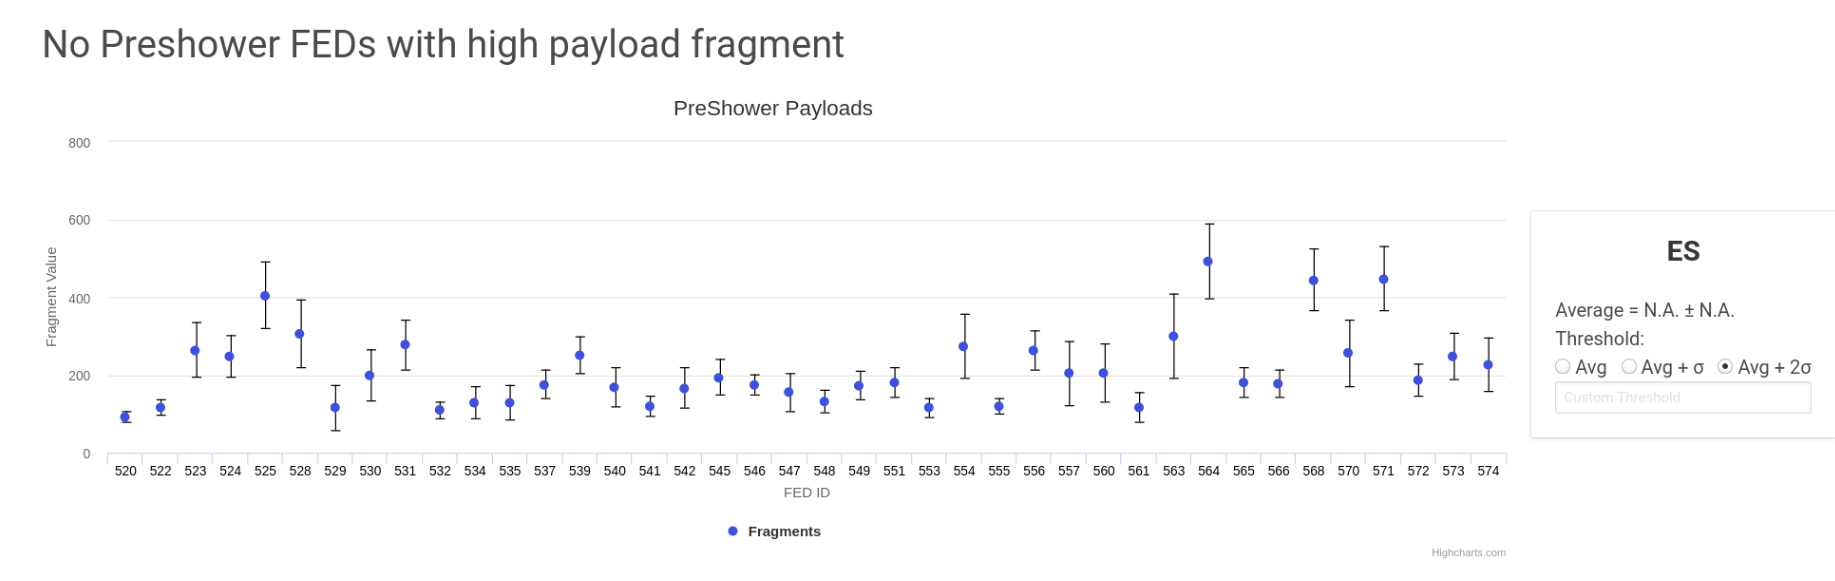
\includegraphics[width=\textwidth]{Images/ECAL_Operations/PayloadMonitor_ES.png}
    \caption{ES payload monitor during a June 2022 full-readout run. On the y-axis, the size of a FED's payload fragment is plotted. On the x-axis, the ES FED number is plotted. Each FED number corresponds to a portion of ES.}
    \label{fig:PayloadMonitor_ES}
\end{figure}

Notably, the payloads in the ECAL barrel appear to be greater on average than the payloads in the ECAL endcaps. This may potentially be due to the fact that there are more readout channels in the EB (61,200 crystals compared to 14,648). 

\subsection{Trigger}

The primary role of the ECAL trigger team is to ensure the smooth operation and proper calibration of ECAL trigger primitive generation. Responsibilities include the identification and masking of noisy or problematic towers, the monitoring of ECAL's contribution to the CMS trigger rate, and the testing and commissioning of new features and protocols for future data-taking periods. A diagram of the ECAL trigger primitive generation path is shown in Figure \ref{fig:ECAL_TCC_Diagram}.

\begin{figure}[H]
    \centering
    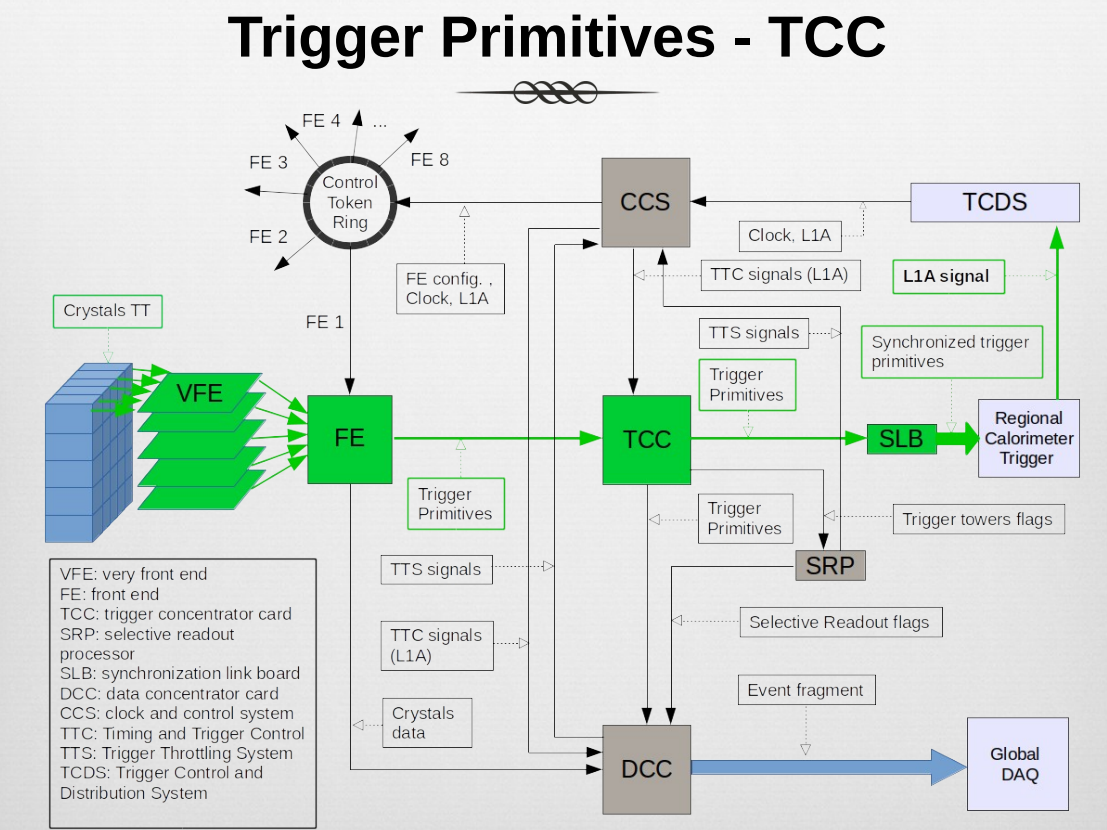
\includegraphics[width=0.85\textwidth]{Images/ECAL_Operations/ECAL_TCC_Diagram.png}
    \caption{ECAL trigger primitive path}
    \label{fig:ECAL_TCC_Diagram}
\end{figure}

While data is first sent to the FE card as described in the previous Section \ref{sec:ECAL_DAQ}, it is stored on the FE electronics buffers while a trigger primitive is formed and sent to the TCC (Trigger concentrator card). The TCC passes the TPs to the calorimeter layers of L1, while the FE waits to receive, or not receive an L1A. 

\subsection{Electronics}

The ECAL electronics team is responsible for the maintenance of the ECAL on- and off- detector electronics. The main off-detector ECAL electronics modules are the TCC (Trigger Concentrator Card), CCS (Clock and Control system), and DCC (Data Concentrator Card). In the ECAL Barrel (EB), there is one TCC, CCS, and DCC per supermodule. By monitoring ECAL electronics, and performing physical maintenance such as the cleaning of electronics fibers or uploading of updated firmware when necessary, the ECAL electronics experts ensure the robustness and ability of the ECAL electronics to take quality data. 

% https://cmsdoc.cern.ch/~jlfaure/OD_Web_Folder/June-02/CCS-veryprelimspecs.pdf

\subsection{Laser and LED}

Due to radiation received by LHC delivered collisions, the transparency of ECAL crystals degrades over time due to radiation damage. A laser correction system is in place in order to measure and correct for losses in ECAL crystal transparency, as shown over the course of LHC Runs 1 and 2 in Figure \ref{fig:ECAL_Laser_History}. It can also be seen that during long shutdown periods without collisions, the ECAL crystals anneal and recover some transparency, as seen by the slight increases in transparency before and after a shutdown period.

\begin{figure}[H]
    \centering
    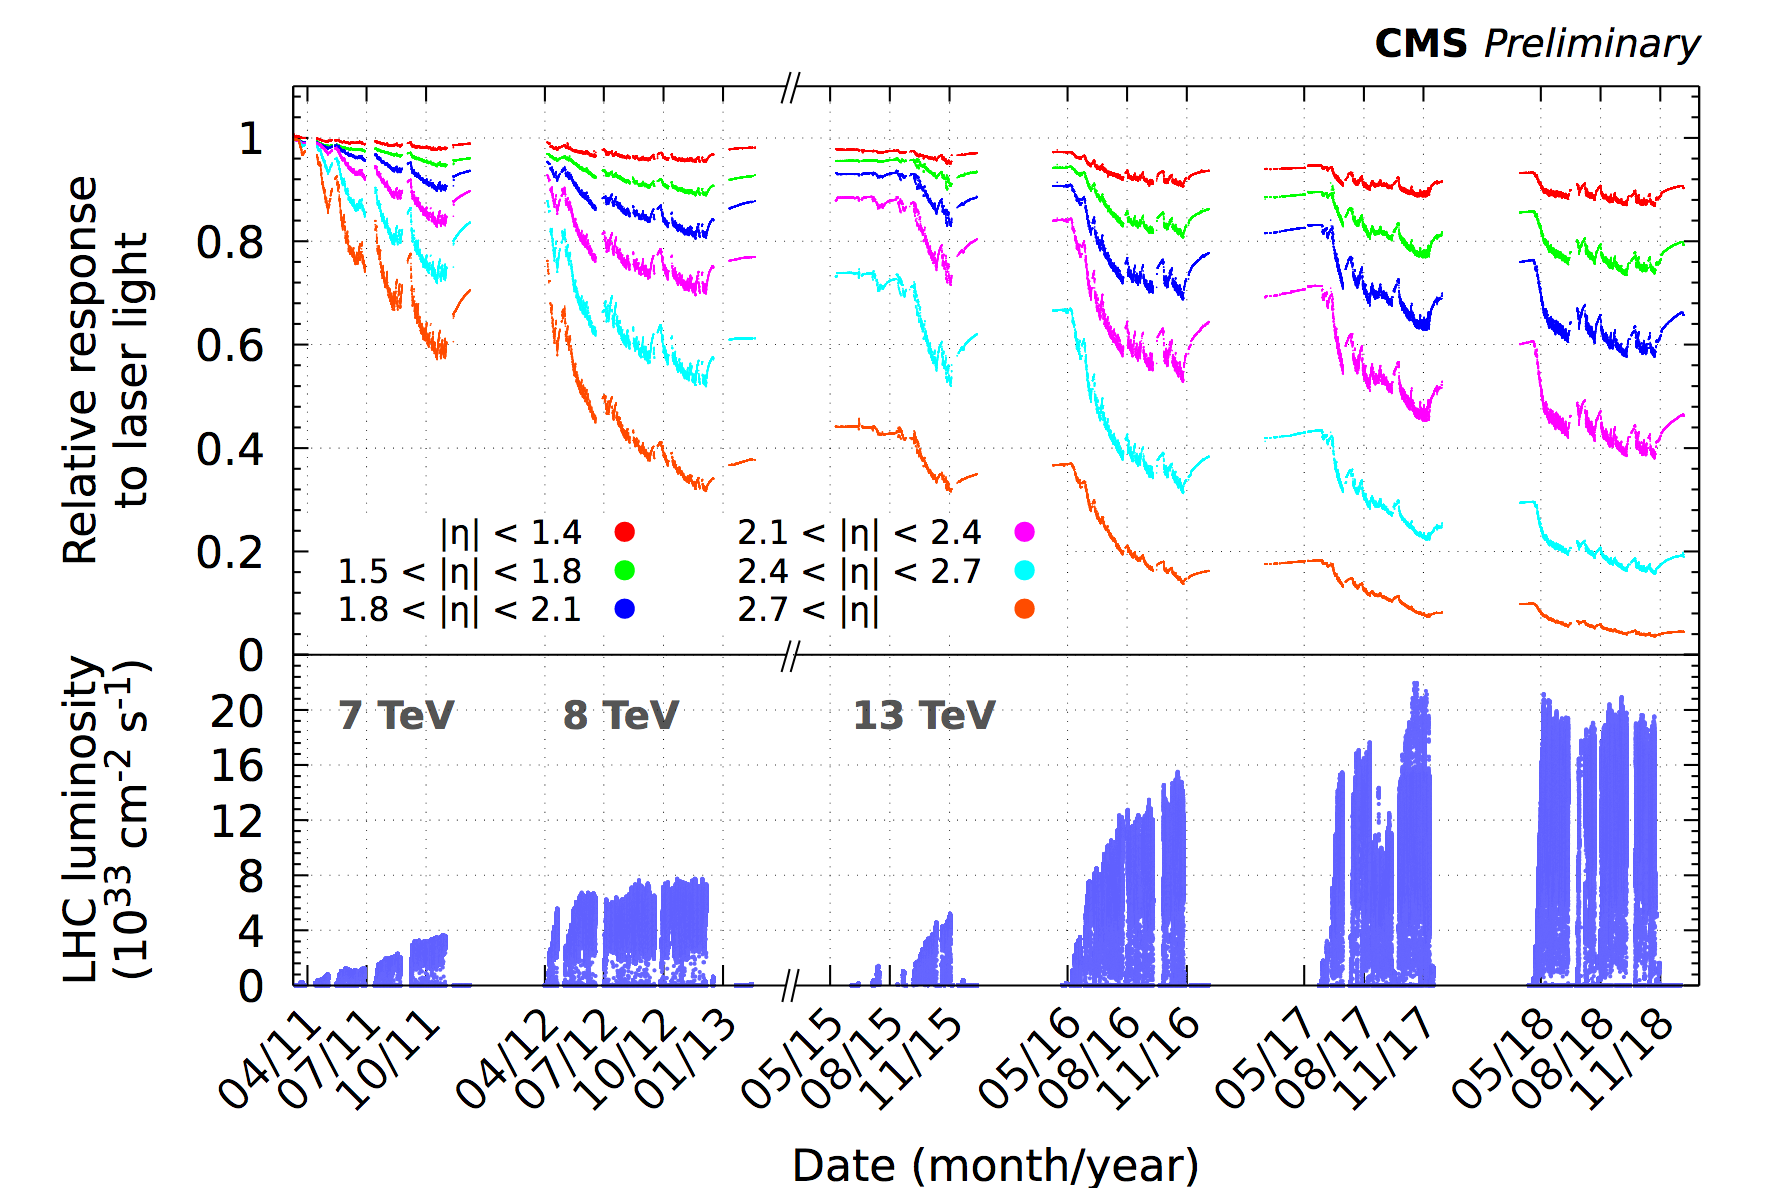
\includegraphics[width=\textwidth]{Images/ECAL_Operations/ECAL_Laser_History.png}
    \caption{ECAL crystal transparency history during LHC Runs 1 and 2.}
    \label{fig:ECAL_Laser_History}
\end{figure}

While similar shapes are observed for different $\eta$ regions of the detector, more radiation is received at higher $\eta$ regions, leading to lower transparency with respect to that from the start of LHC Run 1. In the highest pseudo-rapidity region in the last EE rings 2.7 $< \eta$, the crystals have an average transparency down to $\approx$ 4\% with respect to their original transparency. The high levels of radiation damage in the high $\eta$ regions are consistent with the higher amplitude fractional bias shown in Figure \ref{fig:ampBiasvseta}, and is one of the motivations for replacing the ECAL EE for the Phase-II CMS detector in favor of a new endcap detector called HGCAL (High granularity calorimeter).

An additional transparency measurement is taken by the LED for the ECAL endcaps. The ECAL laser team is responsible for ensuring the smooth operation of the ECAL laser and LED systems, which take crucial measurements to monitor the ECAL crystals and calibrate their outputs. 

\subsection{Data quality monitor} \label{sec:ECAL_DQM}

The purpose of the ECAL Data Quality Monitor (DQM) group is to maintain and develop the ECAL DQM plots used by both the central CMS DQM monitoring page, and the local version used privately by ECAL. An example set of DQM plots is shown in Figure \ref{fig:ECAL_DQM_Plots}. 

\begin{figure}[H]
    \centering
    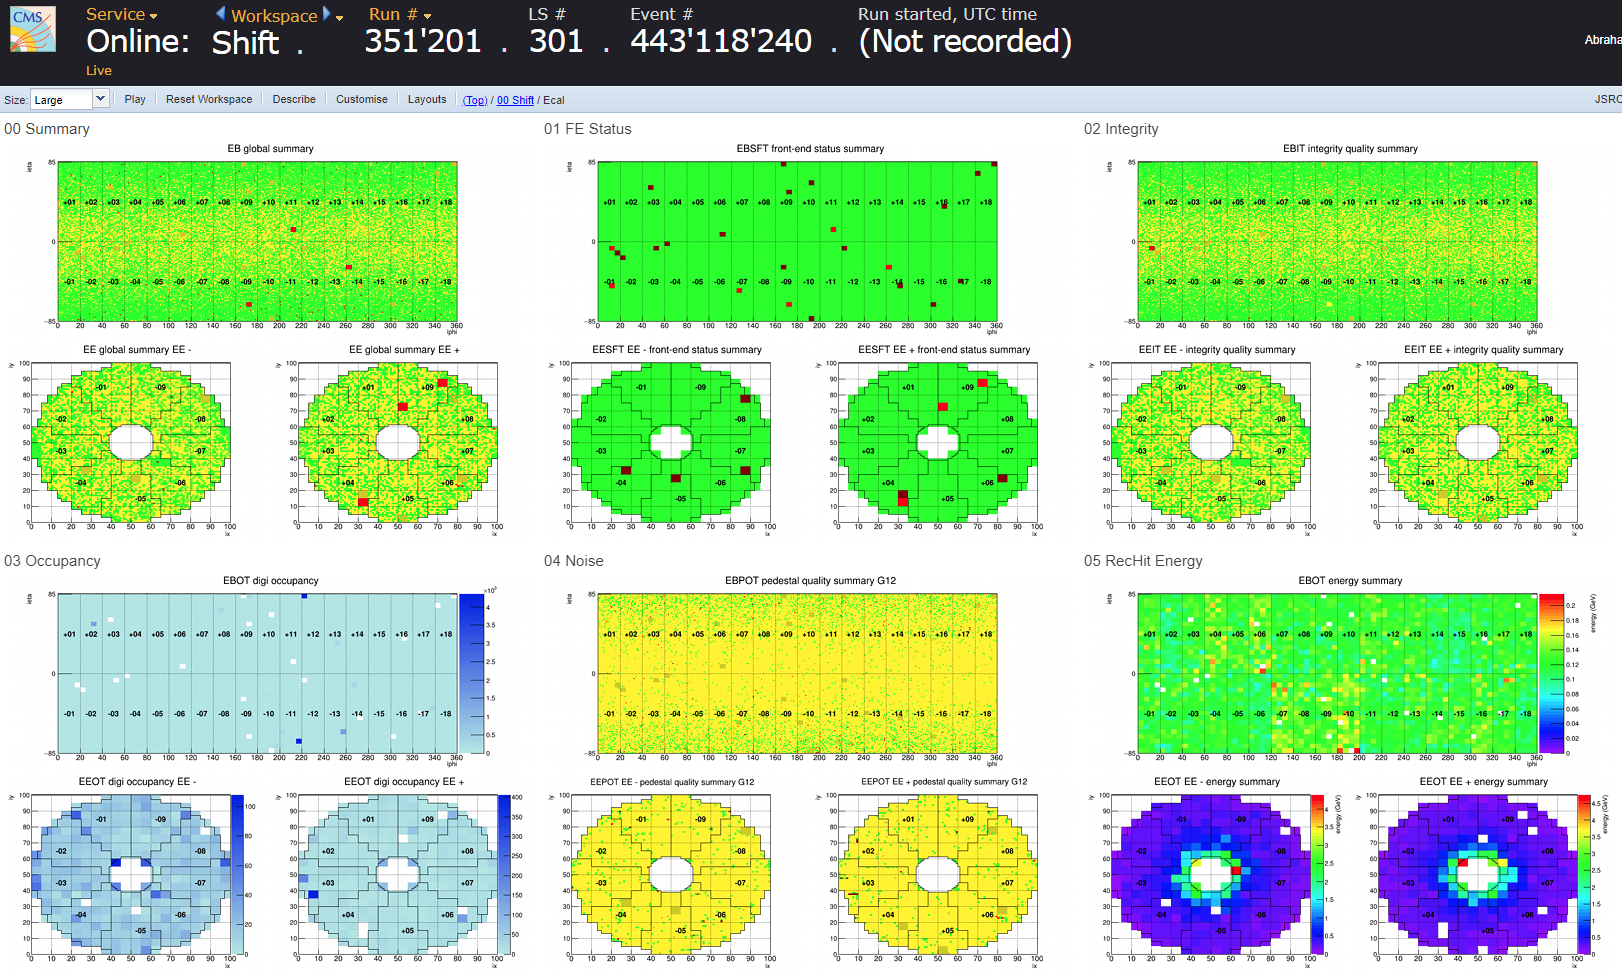
\includegraphics[width=0.75\textwidth]{Images/ECAL_Operations/ECAL_DQM_Plots.png}
    \caption{Example ECAL DQM plots}
    \label{fig:ECAL_DQM_Plots}
\end{figure}

These plots are essential for monitoring the quality of data being taken by ECAL. If large sections of ECAL DQM plots show issues, typically colored red, it may hint at a problem which can be confirmed by going through additional DQM plots in order to better understand the underlying issue. This information would then be propagated to the appropriate ECAL experts in order to take the necessary action, such as fixing a certain piece of hardware or software. It is then checked if a problem has been solved by starting a new run, and confirming that the DQM plots no longer indicate an issue.  

\subsection{Prompt feedback group}

The role of the ECAL Prompt Feedback Group (PFG) is the provide prompt feedback regarding the quality of ECAL data. One of the main roles of the PFG group is to provide daily reports to the entire ECAL operations team, notifying everyone of the general status of ECAL based on a variety of monitoring plots, largely from the DQM previously described in Section \ref{sec:ECAL_DQM}. This daily report is crucial for catching any clear issues in ECAL data-taking, which may affect large portions of CMS data if left un-noticed. 

\subsection{Detector performance group}

The role of the ECAL Detector Performance Group (DPG) includes the maintenance, and improvement in quality of calibration applied to ECAL data. This also includes the tracking of physics performance of the ECAL detector, which can for instance be checked by analyzing the reconstruction of expected physics processes such as $\pi_{0}\rightarrow\gamma\gamma$, shown for runs from a 2022 commissioning period in black and a 2018 data taking period in blue in Figure \ref{fig:piZero_peak_13p6UnstableCollisions}.

\begin{figure}[H]
    \centering
    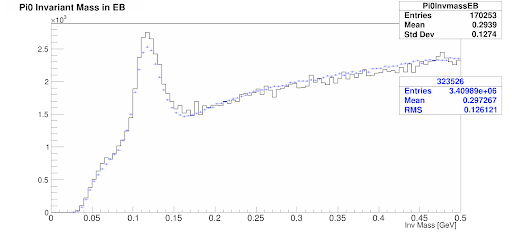
\includegraphics[width=0.85\textwidth]{Images/ECAL_Operations/pi0peak.png}
    \caption{Invariant mass of a diphoton pair from a $\pi_{0}$ candidate in EB during a 2022 commissioning run (black) and 2018 data-taking run (blue).}
    \label{fig:piZero_peak_13p6UnstableCollisions}
\end{figure}
